\section{The Trajectory of a Cannon Ball}

The equations of motion of the system are 
\begin{align}
\ddot{x} &= -k \dot{x} \\
\ddot{y} &= -g - k \dot{y}
\end{align}

where $k = \frac{c_d}{m}$.\\
\\

In state-space form, where $u=[x,y,\dot{x},\dot{y}]^\text{T}$, the system is defined as:
\begin{equation}
\frac{d}{dt} \begin{bmatrix} x \ y \ v_x \ v_y \end{bmatrix} = \begin{bmatrix} v_x \ v_y \ -k v_x \ -g - k v_y \end{bmatrix}
\end{equation}

One may derive explicit solutions for the position of the projectile.

\begin{align}
x(t) &= \frac{v_{x0}}{k} \left( 1 - e^{-kt} \right) \\
y(t) &= \frac{v_{y0}}{k} \left( 1 - e^{-kt} \right) - \frac{g}{k} \left( t - \frac{1}{k}(1 - e^{-kt}) \right)
\end{align}

\begin{minted}{julia}
# --- Define Parameters --- #
m   = 1
θ   = pi/4
v₀  = 10
g   = 1
c   = 1
k = c/m
t_final = 20
t = range(.0, t_final; length=1000)

# --- Initial Conditions --- #
x₀, y₀ = .0, .0
vx₀ = v₀ * cos(θ)
vy₀ = v₀ * sin(θ)

# ===== Part A ===== #

function projectile_analytic(t, vx₀, vy₀, k, g)
    x = (vx₀ / k) * (1 - exp(-k * t))
    y = (vy₀ / k) * (1 - exp(-k * t)) - (g / k) * (t - (1 / k) * (1 - exp(-k * t)))
    return x, y
end

results = projectile_analytic.(t, vx₀, vy₀, k, g)
x_analytic = [r[1] for r in results]
y_analytic = [r[2] for r in results]

# ===== Part B ===== #

# State u = [x, y, dx, dy]
function projectile!(du, u, p, t)
    # Unpack parameter vector
    m, c, g = p
    k = c/m # For convinience
    # Unpack state vector
    x, y, dx, dy = u
    ddy = (- g) + (-k * dy)
    ddx = -k * dx
    du[1] = dx; du[2] = dy
    du[3] = ddx; du[4] = ddy
end

# -- Initial Conditions -- #
u₀  = [x₀, y₀, vx₀, vy₀]
tspan = (.0, t_final)

# Parameter Vector
p = (m, c, g)

# Callback conditon -- stop when y = 0 (hits the floor)

condition(u, t, integrator) = u[2]
affect!(integrator) = terminate!(integrator)
cb = ContinuousCallback(condition, affect!)

problem = ODEProblem(projectile!, u₀, tspan, p)
sol = solve(problem, Tsit5(), callback = cb)

# ===== Part C ===== #
# Evaluate the analytical solution at (t=2)
state_at_2 = [projectile_analytic(2, vx₀, vy₀, k, g)...]
errors = []

tolerances = 10 .^ range(-3, -16, length=20)

for tol in tolerances
    temp_sol = solve(problem, Tsit5(), callback=cb, reltol=tol, abstol=tol)
    
    u_num = temp_sol(2.0)
    pos_num = [u_num[1], u_num[2]]
    
    push!(errors, norm(pos_num - state_at_2))
end
\end{minted}

\begin{figure}[htbp]
     \centering
     % --- Row 1 ---
     \begin{subfigure}[b]{0.45\textwidth}
         \centering
         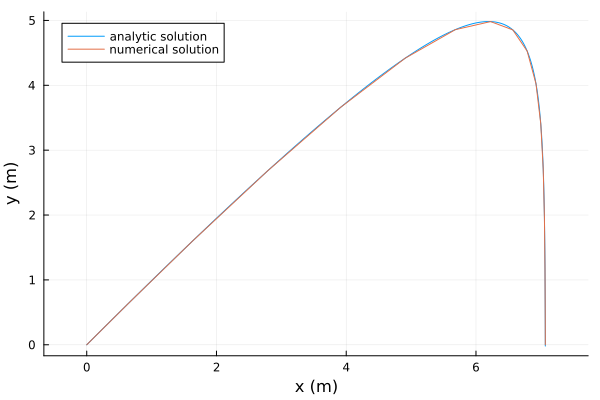
\includegraphics[width=\textwidth]{Problems/Problem9/figures/trajectory.png}
         \caption{Numerical and Analytical Solutions}
         \label{fig:placeholder}
     \end{subfigure}
     \hfill
     \begin{subfigure}[b]{0.45\textwidth}
         \centering
         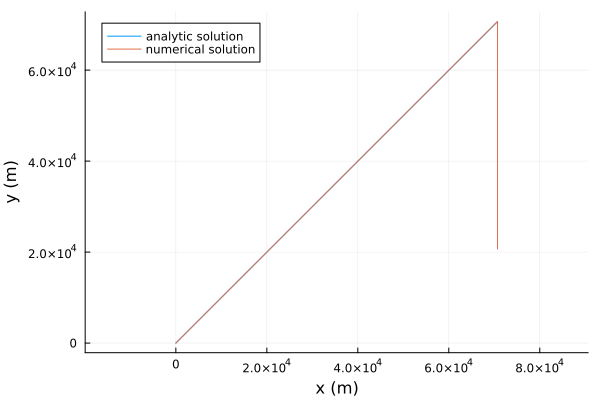
\includegraphics[width=\textwidth]{Problems/Problem9/figures/large_v.png}
         \caption{Trajectory as $v \xrightarrow{} \infty$}
         \label{fig:placeholder}
     \end{subfigure}

    \caption{Projectile Trajectories}
\end{figure}

\begin{itemize}
    \item \textbf{Trajectory Matching:} The numerical solution using the \texttt{Tsit5()} integrator shows high visual agreement with the analytical solution. The use of a \texttt{ContinuousCallback} successfully terminates the simulation at the precise moment of ground impact (y=0).
    
    \item \textbf{Convergence:} The error at t=2 was evaluated against varying tolerances. The resulting log-log plot demonstrates that as the local error tolerances (abstol,reltol) are tightened, the global error decreases linearly on a logarithmic scale, confirming the stability and consistency of the solver.
\end{itemize}

\begin{figure}[h!]
    \centering
    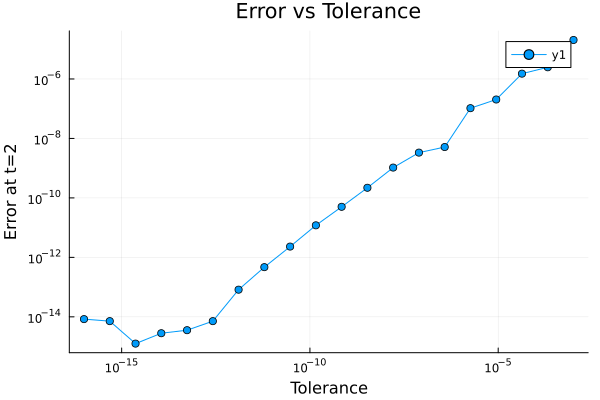
\includegraphics[width=0.5\textwidth]{Problems/Problem9/figures/tolerance_error.png}
    \caption{}
\end{figure}